\documentclass[10pt]{article}

\usepackage{tgschola}
\usepackage[T1]{fontenc}
\usepackage[english]{babel}
\usepackage[dvipsnames]{xcolor}
\usepackage{amsmath}
\usepackage{amssymb}
\usepackage{amsthm}
\usepackage{thmtools}
\usepackage[tmargin=1.0in,bmargin=1.0in,lmargin=0.5in,rmargin=0.5in]{geometry}
\usepackage{graphicx}
\usepackage{caption}
\usepackage{subcaption}
\usepackage{epstopdf}
\usepackage{framed}
\usepackage{fancyhdr}
\usepackage{relsize}
\usepackage{longtable}
\usepackage{array}
\usepackage{titlesec,titletoc}
\usepackage{tabularx}
\usepackage{bbding}
\usepackage{enumitem}
\usepackage{cancel}
\usepackage[font={small,it}]{caption}
%\usepackage[figurename=Fig. ]{caption}
\usepackage{morefloats}
\usepackage{scalerel}
\usepackage{ulem}
\usepackage{makeidx}
\allowdisplaybreaks
\graphicspath{{Figures/}}
\definecolor{special}{rgb}{0.5, 0.5, 0.5}
\definecolor{special2}{rgb}{0.25, 0.25, 0.25}
\definecolor{crimson}{rgb}{0.79, 0.0, 0.09}
\definecolor{gray}{rgb}{0.5,0.5,0.5}

\usepackage[colorlinks=true,linkcolor=crimson,citecolor=crimson,urlcolor=blue,pageanchor=true]{hyperref}
\hypersetup{linktocpage=true,
            pdfstartview=FitV,
            breaklinks=true,
            pdfpagemode=UseNone,
            pdfpagemode=UseOutlines,
            plainpages=false,
            bookmarksnumbered,
            bookmarksopen=true,
            bookmarksopenlevel=1,
            hypertexnames=true,
            pdfhighlight=/O,
            pdfauthor={Nick Vasios},
            pdfkeywords={},
            pdfcreator={pdfTeXify},
            pdfproducer={LaTeX with hyperref}}

\usepackage{listings}
\lstset{language=Matlab,
  morecomment=[l]{!\ }% Comment only with space after !
}

\definecolor{codegreen}{rgb}{0,0.6,0}
\definecolor{codegray}{rgb}{0.5,0.5,0.5}
\definecolor{codepurple}{rgb}{0.4,0,0.7}
%\definecolor{backcolour}{rgb}{0.9,0.9,0.9}
\definecolor{backcolour}{rgb}{0.95,0.95,0.9}

\lstdefinestyle{mystyle}{
    backgroundcolor=\color{backcolour},
    commentstyle=\color{codegreen},
    keywordstyle=\color{magenta},
    numberstyle=\tiny\color{codegray},
    stringstyle=\color{codepurple},
    basicstyle=\footnotesize,
    breakatwhitespace=false,
    breaklines=true,
    captionpos=b,
    keepspaces=true,
    numbers=none,
    numbersep=5pt,
    showspaces=false,
    showstringspaces=false,
    showtabs=false,
    tabsize=2
}
\lstset{style=mystyle}


\titleformat{\chapter}
  {\LARGE\bfseries\color{crimson}}{\thechapter.}{0.3em}{\color{black}\vspace{-2.5em}}
\titleformat{\section}
  {\Large\bfseries\color{crimson}}{\thesection.}{0.3em}{\color{black}\vspace{-1em}}
\titleformat{\subsection}
  {\large\bfseries\color{crimson}}{\thesubsection.}{0.3em}{\color{black}\vspace{-.8em}}%
\titleformat{\subsubsection}
  {\bfseries\color{crimson}}{\thesubsubsection.}{0.3em}{\color{black}\vspace{-.7em}}

\fancypagestyle{plain}{\fancyhead{}\renewcommand{\headrulewidth}{0pt}} 
\pagestyle{fancy}
\renewcommand\thefootnote{\textcolor{red}{\arabic{footnote}}}
\renewcommand{\headrulewidth}{0.5pt}
\renewcommand{\footrulewidth}{0.5pt}
\parskip 7.2pt
\parindent 8pt
\addtolength{\headheight}{3pt}
\renewcommand{\sectionmark}[1]{\markright{\thesection\ #1}}
\renewcommand{\thesubsection}{\thesection.\arabic{subsection}}
\renewcommand{\thesubsubsection}{\thesubsection.\alph{subsubsection}}
\setcounter{tocdepth}{3}
\setcounter{secnumdepth}{3}
\fancyhf{}
\fancyhead[LE,RO]{\thepage}
\fancyhead[LO]{\nouppercase\rightmark}
\fancyhead[RE]{\nouppercase\leftmark}
\PassOptionsToPackage{normalem}{ulem}
\makeindex
\makeatletter

    \setlength{\headheight}{15pt}
    %\numberwithin{figure}{section}
    \renewcommand{\baselinestretch}{1}
    \pagestyle{fancy}
    \addto\captionsenglish{\renewcommand{\contentsname}{Table of Contents}}

\makeatother

    \newcommand{\tocandfigures}{
    \rule[0ex]{1\columnwidth}{0.5pt}
    \begin{flushright}
    \textit{Last Revision: \today}
    \end{flushright}
    \noindent
    \begin{flushleft}
        \makeatletter
        \makeatother
        %\setcounter{page}{1}
        %\setcounter{secnumdepth}{0} %Hide section number in header
    \end{flushleft}
    \tableofcontents
    \noindent
    \begin{flushleft}
        \rule[0.5ex]{1\columnwidth}{.5pt}
        \par
    \end{flushleft}
    \noindent
    \begin{flushleft}
        \newpage{}
        \par
    \end{flushleft}
}
%
%
%
%
    \newcommand{\doabstract}[1]{
        \sectionmark{Abstract}
        \begin{abstract}
            \noindent
            \textit{
            #1
            }
        \end{abstract}
    }

%\setlength\parindent{0pt}


%---------------------------------------------------------------------------
% Custom Definitions for User Name, Course Code and Title, Instructor, etc.
%
\newcommand{\thiscoursecode}{AM 207}
\newcommand{\thiscoursename}{Advanced Scientific Computing}
\newcommand{\thiscoursenameb}{Stochastic Methods for Data Analysis, Inference and Optimization}
\newcommand{\thisprof}{ Verena Kaynig-Fittkau $\&$ Pavlos Protopapas}
\newcommand{\thistf}{Giri Gopalan}
\newcommand{\me}{Karen Yu, Nick Vasios, Thibaut Perol}
\newcommand{\thisterm}{Spring 2016}
%---------------------------------------------------------------------------
%###########################################################################
%---------------------------------------------------------------------------
%                           Code for the Front Page
%
\newcommand{\notefront} {
\begin{center}
    \includegraphics[width=2cm]{SEAS_S}\\[8pt]
    \textbf{\Huge{\thiscoursecode}}{\Huge \\[8pt]}
    {\large{\noun{\thiscoursename}}}\\[8pt]
    {\large{\noun{\thiscoursenameb}}}\\[8pt]
    {{\noun {Harvard John A. Paulson School of Engineering and Applied Sciences}}}
\end{center}
}
%---------------------------------------------------------------------------
%###########################################################################
%---------------------------------------------------------------------------


\newcommand{\no}{\noindent}
\newcommand{\pr}{\partial}
%
\def\beq#1\eeq{\begin{equation}#1\end{equation}}
\def\beqa#1\eeqa{\begin{eqnarray}#1\end{eqnarray}}
\def\beqas#1\eeqas{\begin{eqnarray*}#1\end{eqnarray*}}

\def\blst#1\elst{\begin{lstlisting}#1\end{lstlisting}}



% Quick Underbrace (Math Mode)
\newcommand{\ub}[1]{\underbrace{#1}}

% Quick Underbrace with text (Text Mode)
\newcommand{\ubt}[2]{$\underbrace{\mbox{#1}}_{\mbox{#2}}$}

% Combination Notation (Choose n from p) (Math Mode)
\newcommand{\comb}[2]{{#1 \choose #2}}

% Easy Piecewise function
% 1: Case 1
% 2: Domain for case 1
% 3: Case 2
% 4: Domain for case 2
\newcommand{\piecewise}[4]{\left\{
     \begin{array}{lr}
       #1 & \mbox{#2} \\
       &\\ #3 & \mbox{#4}
     \end{array}
   \right.}

% Easy Slanted Text
\newcommand{\noun}[1]{\textsc{#1}}
% Easy Text TT
\newcommand{\tc}[1]{\texttt{#1}}

% Easy <math>
\newcommand{\sip}[2]{\langle #1 , #2 \rangle}


% Small Greek Letter Shortcuts
\renewcommand\a{\alpha}
\renewcommand\v{\beta}
\newcommand\g{\gamma}
\renewcommand\d{\delta}
\newcommand\e{\epsilon}
\newcommand\ve{\varepsilon}
\def\k{\kappa}
\renewcommand\l{\lambda}
\newcommand\ldot{\dot{\lambda}}
\newcommand\m{\mu}
\newcommand\s{\sigma}
\renewcommand\t{\tau}
\renewcommand\th{\theta}
\newcommand\z{\zeta}
\newcommand\om{\omega}
\newcommand\ups{\upsilon}

% Some Capital Greek Letter Shortcuts
\newcommand\D{\Delta}
\newcommand\F{\Phi}
\renewcommand\L{\Lambda}
\newcommand\Sig{\Sigma}
\def\Om{\Omega}

% Bold Symbols for Vectors and Tensors
\newcommand\baa{\boldsymbol{\alpha}}
\newcommand\bbe{\boldsymbol{\beta}}
\newcommand\bfdel{\boldsymbol{\delta}}
\newcommand\bee{\boldsymbol{\epsilon}}
\newcommand\bve{\boldsymbol{\varepsilon}}
\newcommand\bfeta{\boldsymbol{\eta}}
\newcommand\bkappa{\boldsymbol{\kappa}}
\newcommand\bmi{\boldsymbol{\mu}}
\newcommand\bfxi{\boldsymbol{\xi}}
\newcommand\bs{\boldsymbol{\sigma}}
\newcommand\bom{\boldsymbol{\omega}}
\newcommand\bedot{\dot{\boldsymbol{\epsilon}}}
\newcommand\bGamma{\bf\Gamma}
\newcommand\bDel{\bf\Delta}
\newcommand\bPi{\boldsymbol{\Pi}}
\newcommand\bSig{\boldsymbol\Sigma}
\newcommand\bPhi{\boldsymbol{\Phi}}
\newcommand\bOm{\boldsymbol{\Omega}}
\newcommand\bgrad{\boldsymbol{\nabla}}
\newcommand\cor{\hat{\bs}}
\newcommand\ba{{\bf a}}
\newcommand\bb{{\bf b}}
\newcommand\bc{{\bf c}}
\newcommand\bff{{\bf f}}
\newcommand\bd{{\bf d}}
\newcommand\be{{\bf e}}
\newcommand\bg{{\bf g}}
\newcommand\bh{{\bf h}}
\newcommand\bj{{\bf j}}
\newcommand\bk{{\bf k}}
\newcommand\bl{\boldsymbol{l}}
\newcommand\bm{{\bf m}}
\newcommand\bn{{\bf n}}
\newcommand\bp{{\bf p}}
\newcommand\br{{\bf r}}
\newcommand\bx{{\bf x}}
\newcommand\by{{\bf y}}
\def\bq{{\bf q}}
\newcommand\bss{{\bf s}}
\newcommand\bt{{\bf t}}
\newcommand\bu{{\bf u}}
\newcommand\bv{{\bf v}}
\newcommand\bw{\boldsymbol{w}}
\newcommand\bups{\boldsymbol{\upsilon}}
\newcommand\btau{\boldsymbol{\tau}}
\newcommand\bwv{\{\boldsymbol{w}^{*}\}}
\newcommand\bwt{\{\boldsymbol{w}\}^T}
\newcommand\bwvt{\{\boldsymbol{w}^{*}\}^T}
\newcommand\brho{\boldsymbol{\rho}}
\newcommand\blam{\boldsymbol{\lambda}}
\newcommand\bA{{\bf A}}
\newcommand\bB{{\bf B}}
\newcommand\bC{{\bf C}}
\newcommand\bD{{\bf D}}
\newcommand\bE{{\bf E}}
\newcommand\bF{{\bf F}}
\newcommand\bG{{\bf G}}
\newcommand\bH{{\bf H}}
\newcommand\bI{{\bf I}}
\newcommand\bJ{{\bf J}}
\newcommand\bK{{\bf K}}
\newcommand\bL{{\bf L}}
\newcommand\bM{{\bf M}}
\newcommand\bN{{\bf N}}
\newcommand\bP{{\bf P}}
\newcommand\bQ{{\bf Q}}
\newcommand\bR{{\bf R}}
\newcommand\bS{{\bf S}}
\newcommand\bT{{\bf T}}
\newcommand\bU{{\bf U}}
\newcommand\bV{{\bf V}}
\newcommand\bW{{\bf W}}
\newcommand\bX{{\bf X}}
\newcommand\bY{{\bf Y}}
\newcommand\bZ{{\bf Z}}
\newcommand\bOM{{\bf \Omega}}
\newcommand\bPsi{{\bf \Psi}}
\newcommand\bLam{{\bf \Lambda}}
\newcommand\bzero{{\bf 0}}
% Other
\newcommand\Ccal{\mathcal{C}}
\newcommand\Dcal{\mathcal{D}}
\newcommand\Ical{\mathcal{I}}
\newcommand\bLcal{\boldsymbol{\mathcal{L}}}
\newcommand\bMcal{\boldsymbol{\mathcal{M}}}
\newcommand\bKcal{\boldsymbol{\mathcal{K}}}
\newcommand\bJcal{\boldsymbol{\mathcal{J}}}
\newcommand\bCcal{\boldsymbol{\mathcal{C}}}
\newcommand\bIcal{\boldsymbol{\mathcal{I}}}
\newcommand\bDcal{\boldsymbol{\mathcal{D}}}
\newcommand\Lcal{\mathcal{L}}
\newcommand\Mcal{\mathcal{M}}


\newcommand{\union}{\cup}
\newcommand{\inter}{\cap}

% Very useful shortcuts for sets
\newcommand{\nset}[1]{#1_1,\ldots,#1_n}
\newcommand{\setk}[2]{#1_1,\ldots,#1_#2}
\newcommand{\bnset}[1]{\{#1_1,\ldots,#1_n\}}
\newcommand{\bset}[2]{\{#1_1,\ldots,#1_#2\}}
\newcommand{\ton}[1]{#1=1,\ldots,n}
\newcommand{\tok}[2]{#1=1,\ldots,#2}

% Operators
\newcommand{\disc}{\operatorname{disc}}
\newcommand{\spn}{\operatorname{Span}}
\newcommand{\rank}{\operatorname{rank}}
\newcommand{\proj}{\operatorname{proj}}
\newcommand{\prp}{\operatorname{perp}}
\newcommand{\tran}[1]{#1^\mathrm{T}}

% Underlines
\newcommand{\ux}{\underline{x}}
\newcommand{\ua}{\underline{a}}
\newcommand{\uu}{\underline{u}}

\theoremstyle{definition}
%\newtheorem{cor}{Corollary}[section]
\newtheorem*{note}{Note}
\newtheorem{notation}{Notation}[section]
\newtheorem{exercise}{Exercise}[section]
\newtheorem*{solution}{Solution}
\newtheorem*{ans}{Answer}

\newcommand{\Lp}{\mathcal{L}^p}

\declaretheorem[name=Theorem,
refname={theorem,theorems},
Refname={Theorem,Theorems},
numberwithin=section]{thrm}

\declaretheorem[name=Lemma,
refname={lemma,lemmas},
Refname={Lemma,Lemmas},
numberwithin=section]{lem}

\declaretheorem[name=\color{crimson} Example,
refname={example,examples},
Refname={Example,Example},
numberwithin=section]{exmp}

\declaretheorem[name=Remark,
refname={remark,remarks},
Refname={Remark,Remarks},
numberwithin=section]{rem}

\declaretheorem[name=Proposition,
refname={proposition,propositions},
Refname={Proposition,Propositions},
numberwithin=section]{prop}

\declaretheorem[name=Definition,
refname={definition,definitions},
Refname={Definition,Definitions},
numberwithin=section]{defn}

\newcommand{\Python}
{
\begin{flushright}
  \textit{Python Example}
\end{flushright}\vspace{-2ex}
}
\newcommand{\var}{\mathrm{var}}
\newcommand{\cov}{\mathrm{cov}}

\DeclareMathOperator*{\Assembly}{\scalerel*{\mathrm{A}}{\Big[}}
\newcommand*\tick{\item[\Checkmark]} 

\usepackage{etoolbox}
\makeatletter
\patchcmd{\chapter}{\if@openright\cleardoublepage\else\clearpage\fi}{}{}{}
\makeatother


\begin{document}
\begin{titlepage}
\thispagestyle{empty}
%
\centering
%
\vspace{-6em}
\includegraphics[width=2.5cm]{SEAS_S}\qquad\qquad\qquad
\qquad\qquad\qquad
\qquad\qquad\qquad
\qquad\qquad\qquad
\qquad\qquad\qquad
\qquad\includegraphics[width=2.9cm]{IACS}\\[-2em]
{\bfseries{\Huge{\thiscoursecode}}}\\[8pt]
{\bfseries\large{\thiscoursename}}\\[8pt]
{\large{\thiscoursenameb}}\\[8pt]
{\noun {Harvard John A. Paulson School of Engineering and Applied Sciences}}\\[6cm]
%%

{\LARGE\bfseries \noun{Energy Disaggregation from Non-Intrusive Load Monitoring}}\\[6pt]
{ \noun{Combinatorial Optimization, Factorial Hidden Markov Model, Convolutional Neural Networks}}\\[7.25cm]

{\me}\\[6pt]
{Instructors: \thisprof} \\[6pt]
{TF: \thistf} \\[6pt]
%
{\noun Spring 2016}\\[6pt]
\noun{Last Revision : \today}
%
%
%
\vfill
\end{titlepage} 

{
\abstract{ \it The forward problem of determining the power consumption of a household given the state of each appliance in that household is a very easy and relatively uninteresting problem. On the other hand, the inverse problem (energy disaggregation) seeks to determine the state of each appliance in a household given the aggregate power consumption and is a much harder and a much more interesting problem. Computational techniques make energy disaggregation possible in a non-intrusive manner informing homeowners on the patters of energy consumption on the basis of appliances, facilitating the application of energy efficiency measures and enabling users to increase savings. Several methods have been employed in an effort to disaggregate the energy varying from brute force deterministic methods (CO) to stochastic methods (FHMM) and neural networks. This study is based on the non intrusive load monitoring toolkit developed specifically for these types of problems and the REDD data set for actual households from 2011. We implement, examine and compare three different disaggregation methods namely a Combinatorial Optimization, a Factorial Hidden Markov Model and a Convolutional Neural Network and we conclude that energy can be disaggregated very accurately with the latter}

}

\section{Introduction}
\hspace{2ex} Energy disaggregation is the procedure that infers the energy consumption of appliances in a household given the total energy consumption from a single meter of that household. In recent years, this field has become increasingly popular as smart meters have begun to deploy and are installed in many households across the world, providing energy consumption data at high temporal resolution. This high resolution data enables the use of computer algorithms to estimate the energy consumption of each appliance in the household without having to install meters on individual appliances (hence, non-intrusive load monitoring). Appliance-specific energy consumption information can be provided to homeowners to encourage adoption of energy efficiency habits and identify the appliances that would result in the most cost savings if replaced with more energy efficient ones. From the electric utility's perspective, the appliance specific information can be used for demand-response programs and also provide information about how their customers are using electricity within their homes.

Research on NILM began in the 1980s with \cite{Hart1985}. In these earlier methods, the patterns in electricity consumption of different appliances were identified by humans and these hand-designed feature extractors were then applied to the aggregate signals. Later works \cite{Neural_Kelly} developed methods to automatically identify appliances and perform disaggregation. The technology has also been monetized by several startups (eg. Bidgeley, PlotWatt).

Several data sets have been released for the purpose of comparing disaggregation methods. The Reference Energy Disaggregation Dataset (REDD) \cite{REDD} was released in 2011 from MIT. It includes data from 6 houses spaning a period of approximately one month for each house and contains sub-metered (appliance-level) data for each household. Due to the cost and intrusiveness of installing appliance-level meters, these datasets tend to have only a few households or span a short period of time.

In an attempt to standardize comparison of different disaggregation methods, \cite{NILMTK} released the Non-intrusive Load Monitoring Toolkit \href{http://nilmtk.github.io}{NILMTK}. NILMTK is an open-source toolkit that provides tools for data processing and evaluation metrics. NILMTK also provides two benchmark disaggregation algorithms, combinatorial optimization (CO) and factorial hidden markov model (FHMM).

In this project, we compare a new approach using convolutional neural networks against the standard CO and FHMM implementations in NILMTK.

\subsection{Data processing}
We use the REDD dataset, which contains data aggregated and sub-metered data from 6 houses. We use the functions provided in \verb NILMTK  to read in the data. In the figure below, we show the aggregated energy consumption of a household (building 2) over a 13 day period as well as the times each individual appliance was on during a period of 1 day.

\begin{figure}[!ht]
  \centering
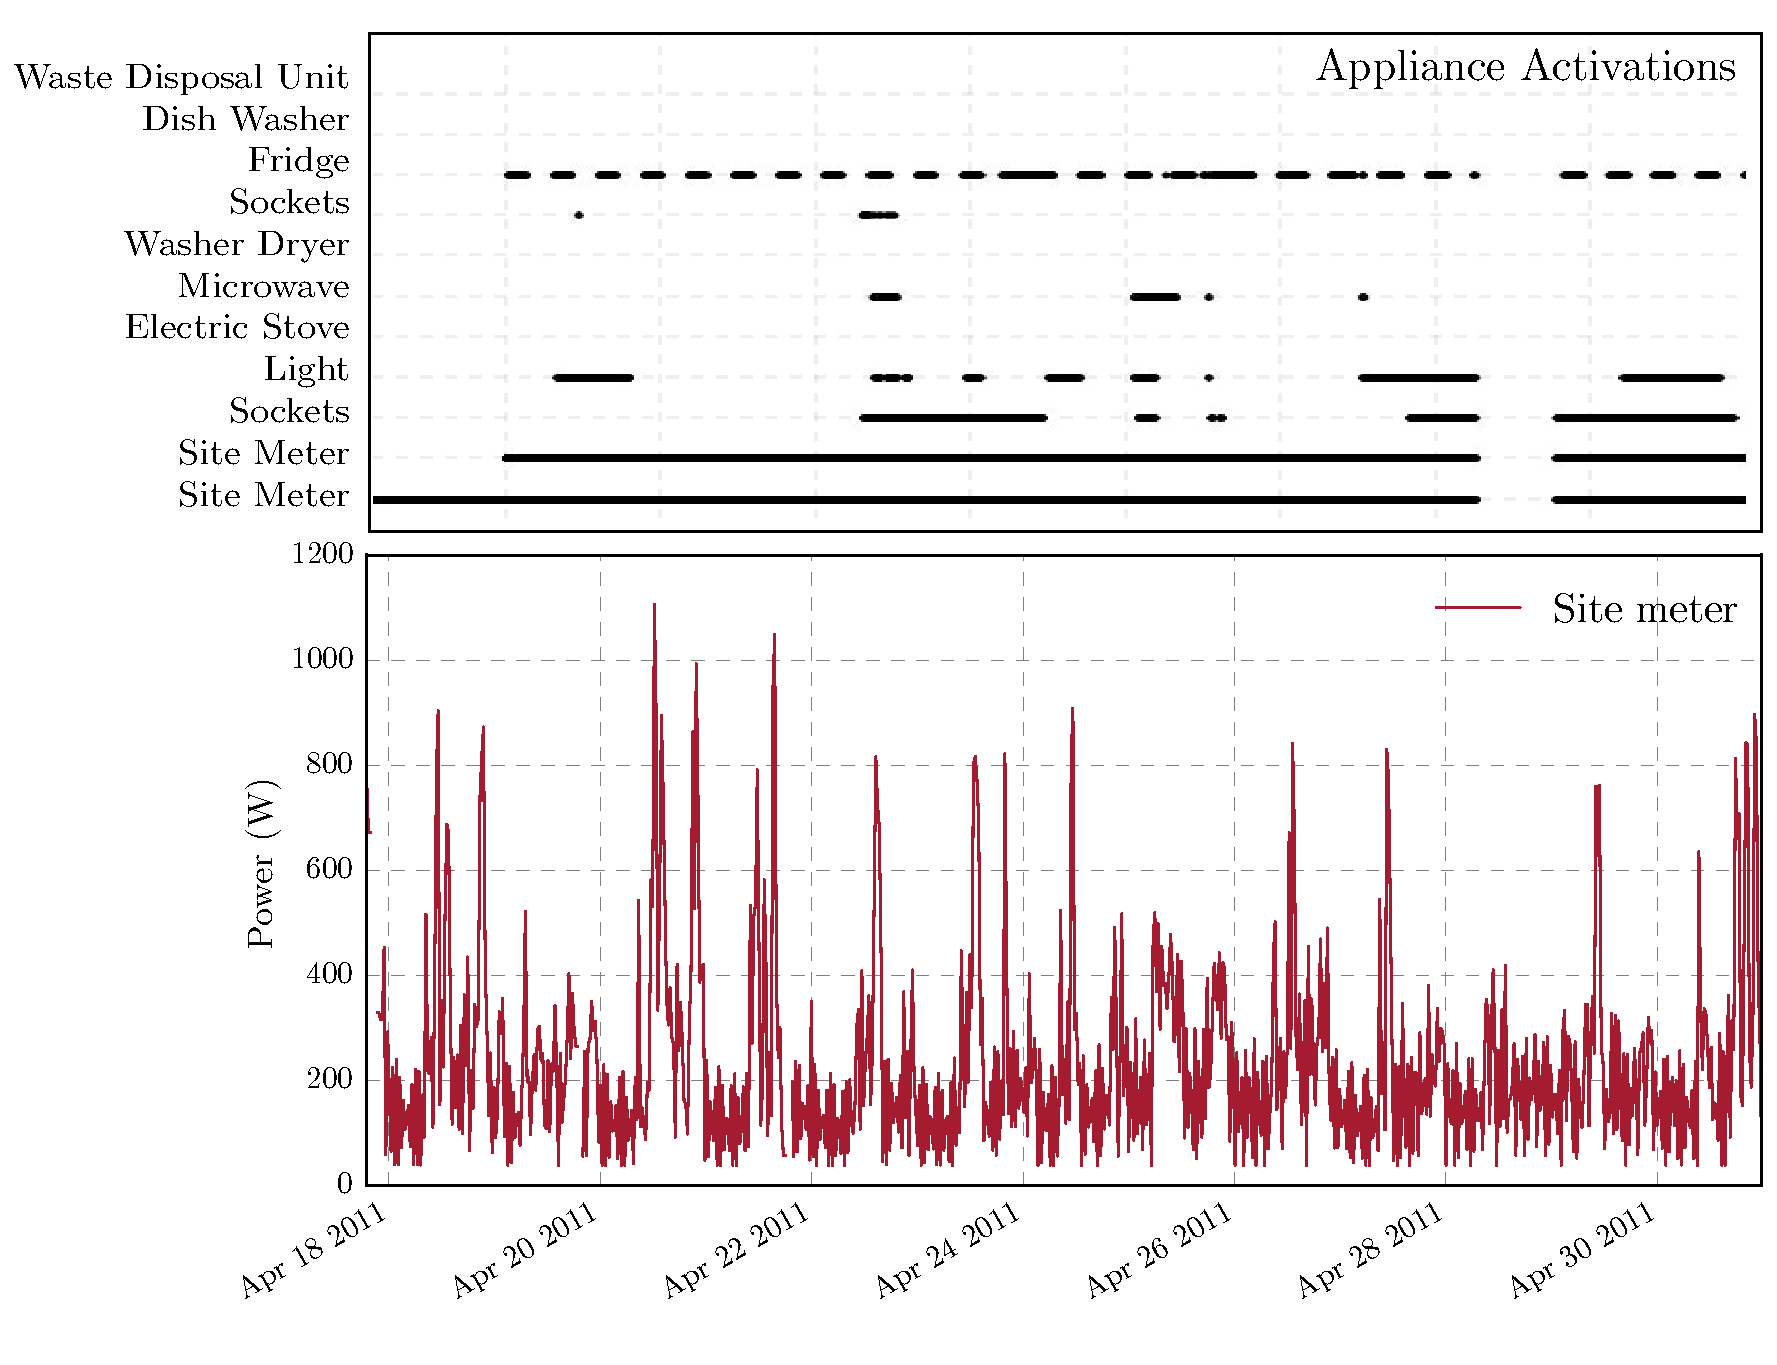
\includegraphics[width=0.6\paperwidth]{Site_Meter.pdf}
  \caption{The aggregate energy consumption of a household (Building 2 in the REDD dataset) along with the activations of the individual appliances}\label{fig:site_meter}
\end{figure}

The data is organized by buildings. Within each building, we can get the electricity meter readings using the \verb .elec  attribute. The \verb .mains  sub-meters refer to the aggregated readings. We can refer to each appliance by giving the appliance as a keyword to \verb data.buildings[building_num].elec[appliance] . Some typical appliances in these households include refrigerators, washter dryers, lights, dish washers, microwaves, and sockets. We decided to use fridge and microwave as the two appliances for which we determine the power consumption because they are used in most households (buildings 1, 2, 3, 5).

The data pipeline is shown in Figure~\ref{fig:pipeline}.

\begin{figure}[!ht]
  \centering
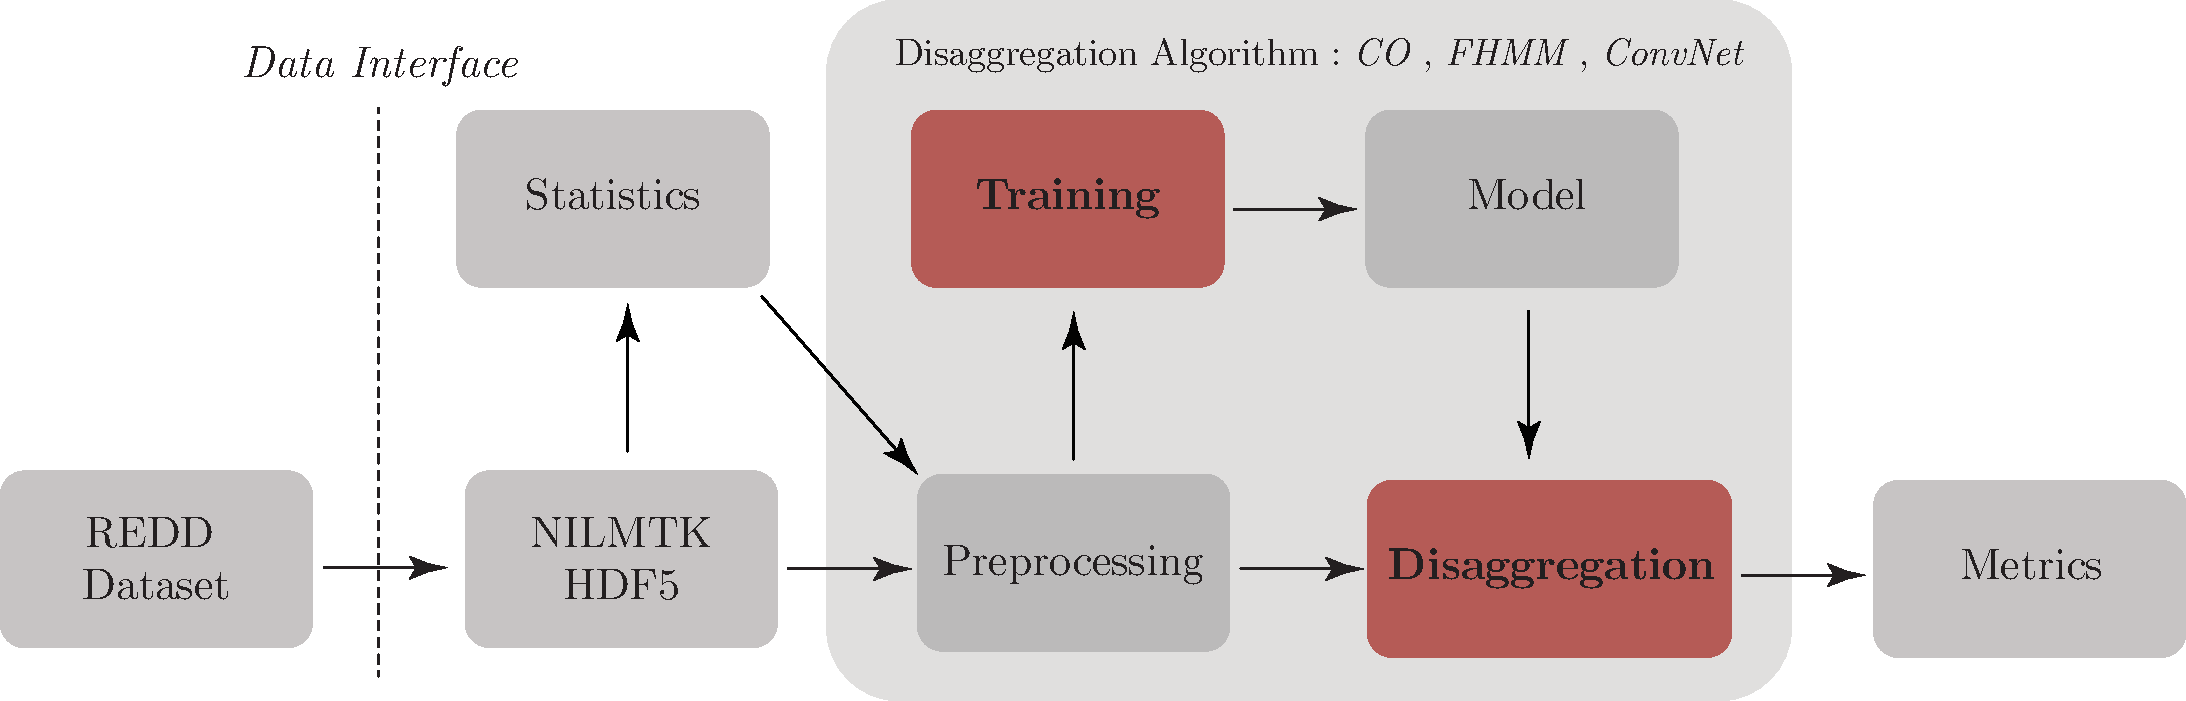
\includegraphics[width=0.6\paperwidth]{NILM_Data_Pipeline.pdf}
  \caption{A graph of the data pipeline used in NILM and the REDD dataset. At each stage of the pipeline, results and data can be
stored to or loaded from disk}\label{fig:pipeline}
\end{figure}

The REDD dataset is first converted to HDF5 format. \verb NILMTK  provides functions to compute statistcs on the dataset as well as preprocessing algorithms. The data from individual meters is then fed into the model for training. After training, the aggregated data can then be fed into the model for disaggregation. \verb NILMTK  also provides functions for computing metrics of how well each disaggregation algorithm performs although we implemented it ourself for the neural network algorithm.

The metrics that we use for comparison of methods are recall, precision, F1, and accuracy, which are created from combinations of the metrics true positives (TP), false positives (FP). false negatives (FN), false negatives (FN), true negatives (TN), number of positives in ground truth (P), and number of negatives in ground truth (N).

\[\mathrm{recall} = \dfrac{TP}{FP + FN}, \hspace{5mm} \mathrm{precision} = \dfrac{TP}{TP + FP}, \hspace{5mm} F1 = 2 \times \dfrac{\mathrm{precision} \times \mathrm{recall}}{\mathrm{precision} + \mathrm{recall}} \hspace{5mm} \mathrm{accuracy} = \dfrac{TP + TN}{P + N}\]

\section{Methods}
%\hspace{2ex} In order to successfully disaggregate the total energy in a household into its components, we need to devise methods that would be able to determine the status (state) of every appliance based on the aggregated demand. Since the goal is to use the methods for energy disaggregation in new households for which only the aggregated data is available, it is necessary to build models of every appliance based on previous experience from other households. For this reason, all of the methods used for this project involve a training stage, where existing data for the energy consumption across all appliances as well as the aggregated consumption are being used to create models for each appliance, based on which the disaggregation would later be possible. However, the training and the disaggregation stages for each method considered in the context of this project are substantially different and are explained in further detail in the sections that follow.


\subsection{Combinatorial Optimization}
\hspace{2ex} One of the most natural way to formulate the inverse problem of energy disaggregation into its appliance components is using Combinatorial Optimization. Since the number of appliances in a household is always finite and discrete as well as the states (on, off, intermediate) of each appliance, the problem could be that of finding the combination of appliance states for each appliance that minimizes the difference between the sum of the predicted appliance power and the observed aggregate power demand. Let us formally state the problem using some notation as follows. We denote with $x_t^{(n)}$ the state of appliance $n$ at time $t$, and with $P_{i}^{(n)}$ the energy  consumption of the same appliance at state $i$. Since the energy consumption of most appliances is not constant over all periods of time, one appliance is possible to have more states than the \textit{ON}, \textit{OFF} ones usually modelled. For instance, an oven/burner appliance may operate in multiple different states for different temperature setups as well as cooking modes. In general, the oven is possible to operate in all of these states during time period and knowing which these states are, makes it easier to spot them in the aggregated data. Using this definitions as well as the ground truth for the aggregated energy consumption $\overline{y}_t$ at time $t$ we can determine the optimal state for each appliance as:
%
\begin{equation}\label{CO_sol_1}
\hat{x}^{(n)}_t=\mathop{\mathrm{argmin}}_{\hat{x}^{(n)}_t}\left|\overline{y}_t-\sum_{n=1}^N{x_t^{(i)}P_{x_t}^{(i)}}\right|=\mathop{\mathrm{argmin}}_{\hat{x}^{(n)}_t}\left|\overline{y}_t-\sum_{n=1}^N{\hat{y}_t^{(n)}}\right|
\end{equation}
%

Despite being mathematically attractive, the formulation described by \eqref{CO_sol_1} is associated with a number of difficulties. The main difficulty is that $P_{i}^{(n)}$ is impossible to be determined across a large number of potentially different houses, not only because of the fact that an appliance may operate in many different states $i$ with different $P_i$ but also because the number and type of appliances are almost never the same in any two households. In addition to this, the appliances in a household are also subject to change in time since some new appliances may be added (i.e. buying a new hairdryer) or removed (i.e. washer breaks down). To make things even worse, the solutions obtained by \eqref{CO_sol_1} are sometimes against our intuition. This may happen because small changes in $\overline{y}$ in a short interval $\D t$ may lead to dramatic changes in $\hat{x}^{(n)}_t$ due to the minimization in \eqref{CO_sol_1}. The reason this is allowed in this formulation, is attributed to the fact that each time slice is a different combinatorial optimization problem and therefore is not related with adjacent time slices, thus allowing for much different solutions in short periods of time. Our intuition however, suggests that is not at all likely that many appliances can change states all together in short periods of time. Last but not least, this particular formulation of the CO algorithm resembled the subset sum problem and is therefore NP-complete \cite{NILMTK,Hart}. The computational complexity of this algorithm is of the order $O(TK^N)$, where N is the number of appliances, K is the number of appliance states and $T$ is the number of time slices. This means that the complexity scales exponentially with the number of appliances making the disaggregation computationally intractable for large number of modelled appliances.

\begin{figure}[!ht]
  \centering
  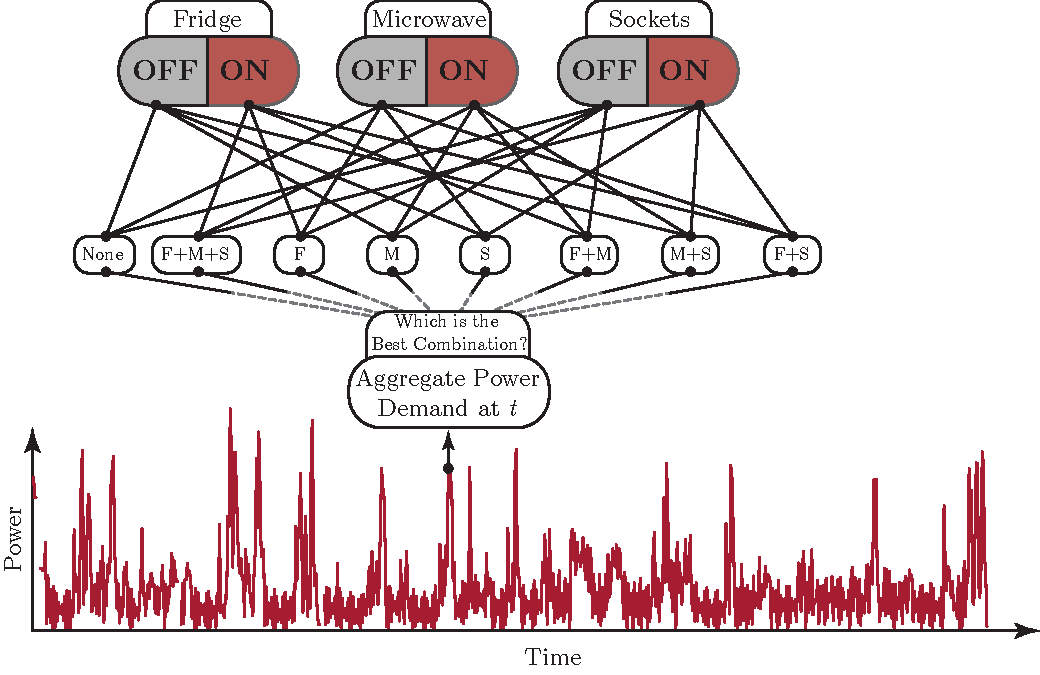
\includegraphics[width=0.75\textwidth]{Combinatorial}
  \caption{A schematic illustration of the possible combinations for appliance states in the simplistic case of 3 appliances with 2 states each. Recall that this selection of the optimal combination has to be performed at every time slice of the time window}\label{fig:comb}
\end{figure}

%

Figure~\ref{fig:comb} shows a typical step in the disaggregation using Combinatorial Optimization in the case of 3 appliances with only 2 states for each one. Clearly, it is evident that as the number of states goes up, which is a natural generalization to make in order to model each appliance more naturally, the computational complexity blows up.

The training step in the Combinatorial Optimization algorithm involves the problem of classifying the energy consumption of appliances in order to determine the states of each. The clustering is performed using the K-Means algorithm and the number of clusters to be used in the clustering can be easily modified by the user. However, as already mentioned, the computational cost scales exponentially with the number of states and therefore if there are many appliances on which we need to train on, then it is advised to use only the basic ON, OFF states and therefore only 2 clusters. Once the states are determined in training, the algorithm can successfully disaggregate the energy to the appliances on which it was trained on.
\subsection{Factorial Hidden Markov Model}
Factorial hidden markov models (FHMM) are an extension to hidden markov models (HMM) where the hidden state is factored into multiple state variables \cite{Ghahraani}. In a hidden markov model, the observed states of the system are the aggregated power consumption of the household. The hidden states are the states of each appliance. This is shown in the diagram below.

\begin{figure}[!ht]
  \centering
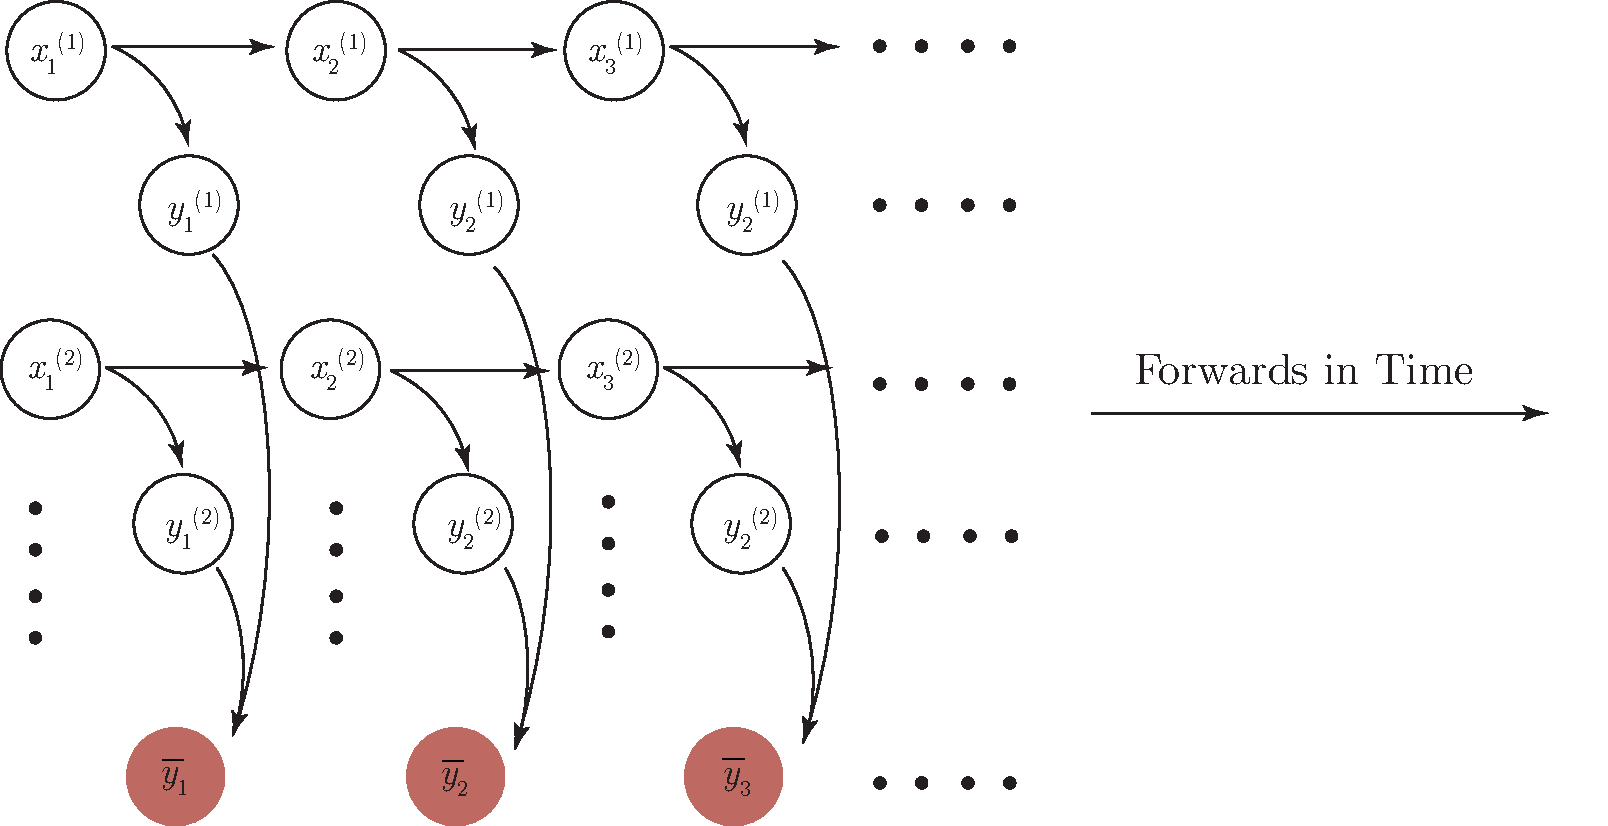
\includegraphics[width=0.8\textwidth]{FHMM.pdf}
  \caption{A typical states diagram for the Factorial Hidden Markov Model \cite{REDD}}\label{fig:HFMM}
\end{figure}

In the above diagram, $\overline{y}_t$ is the observed state (aggregate power consumption) at time $t$, $y_t^{(i)}$ is the power consumption of appliance $i$ at time $t$ (used only in training), and $x_t^{(i)}$ is the hidden state of appliance $i$ at time $t$. Since the observed state is continuous, the emission probabilities are modeled with a Gaussian distribution:

\[P(y_t|x_t^{(1:N)}) = \mathcal{N} \left(\sum_{i=1}^N \mu^{(i)}, \Sigma \right) \]

where the mean is the sum of the means of the individual appliances. The transition probabilities can be factored as

\[P(x_t^{(1:N)}|x_{t-1}^{(1:N)}) = \prod_{i=1}^{N} P(x_t^{(i)}|x_{t-1}^{(i)})\]

and the transition probabilities for each individual appliance follow a multinomial distribution. The model also needs an initial probability distribution, $\pi_0$ which also follows a multinomial probability distribution.

In the NILMTK implementation, the \verb train_across_buildings  function takes as input the sub-metered data for each house, a list of the appliances we want to train for, and a list of the houses we want to include in the training set. The sub-metered data for each appliance is then combined into an array that includes all training houses. An HMM with Gaussian emissions is built for each appliance using the \verb GaussianHMM  function in the \verb hmmlearn  package. The parameters (transition and emission probabilities) for this HMM is then trained using the \verb fit  function from \verb hmmlearn , which uses expectation-maximization (EM) to find the optimal parameters. In the original NILMTK implementation, there are two hidden states for each appliance to represent on and off states. We modify the function to allow for a user-specified number of hidden states.

Once these parameters are fit for all appliances, they are combined to form the FHMM. The FHMM has a hidden state for every possible combination of states. To create the combined emission matrix, the mean power consumption for each appliance is summed (if the fridge comsumes 0.5W while off and 150W while on, and a microwave consumes 3 W while off and 350 W while on, then the states would be 3.5 W for both devices off, 153 W for fridge on, microwave off, 350.5W for fridge off, microwave on, and 500 W for both devices on). To create the combined transition matrix, we take the product of the transition probabilities of individual appliances. A new \verb GaussianHMM  model is created using these combined parameters.

To disaggregate (infer the hidden states), the \verb predict  function of \verb hmmlearn  is used, which has the option of using the Viterbi algorithm or maximum a posteriori (MAP) to decode the most likely state sequence.

\section{Convolutional Neural Network (ConvNet)}
The implementation of the method presented in this section can be found in the \href{https://github.com/tperol/am207-NILM-project/blob/master/Report_convnet.ipynb}{notebook}. However the main codes are available in a separate \href{https://github.com/tperol/neuralnilm}{repository} to keep this final repository clean. Most of the codes for preprocessing of the data are borrowed from \href{https://github.com/JackKelly/neuralnilm}{Jack Kelly repository} that was forked. However the implementation of the python generator for the data augmentation on CPU, the ConvNet implementation (trained on GPU) and post processing for the metrics are our own implementation.

\subsection{ConvNet introduction}
Convolutional Neural Networks are similar to ordinary Neural Networks (multi-layer perceptrons). Each neuron receive an input, perform a dot product with its weights and follow this with a non-linearity (here we only use ReLu activation functions). The whole network has a loss function that is here the Root Mean Square (RMS) error (details later). The network implements the 'rectangle method'. From the input sequence we invert for the start time, the end time and the average power of only one appliance (see Figure~\ref{convnet_architecture}).

\begin{figure}
\begin{center}
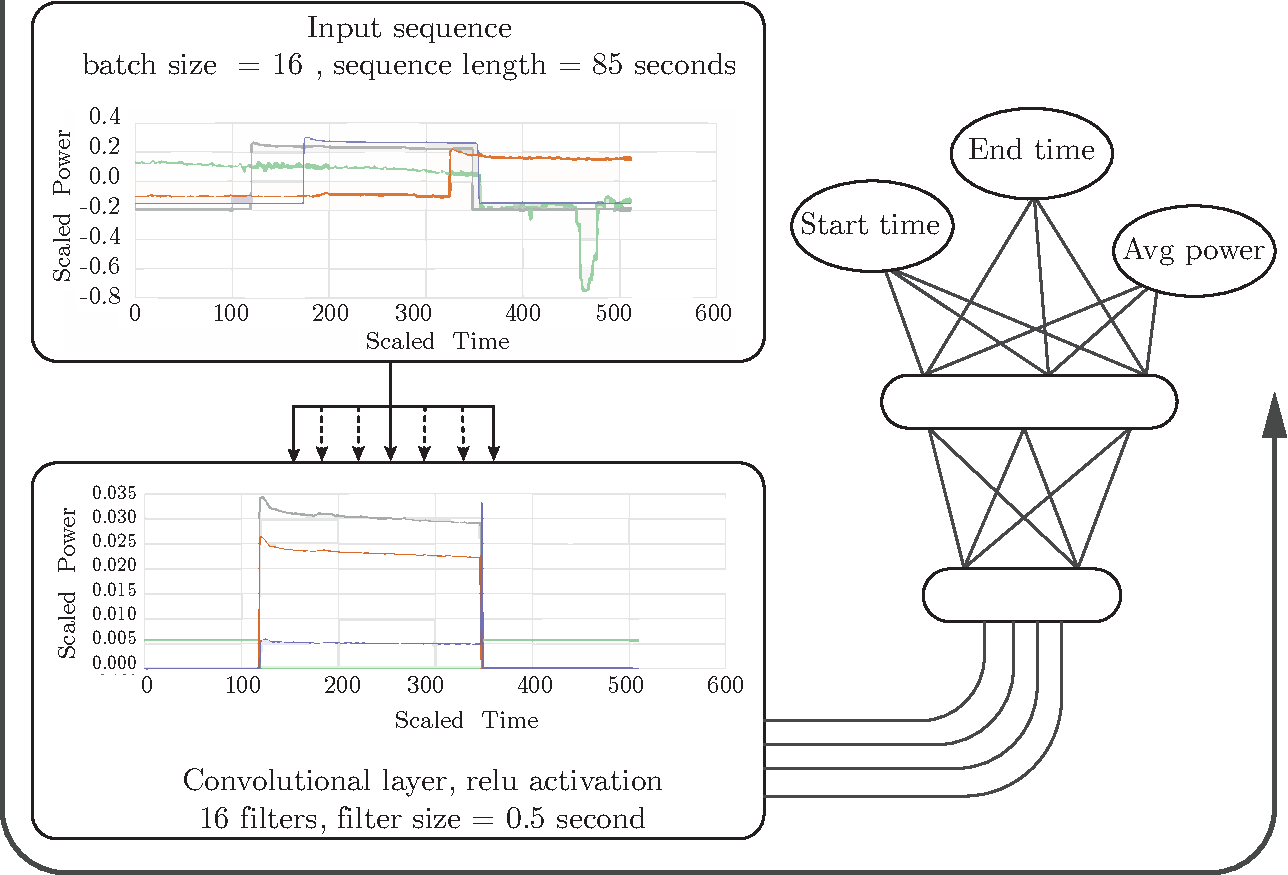
\includegraphics[width=29 pc]{convnet_architecture}
\caption{A schematic representation of the architecture of the convolutional neural network}
\label{convnet_architecture}
\end{center}
\end{figure}

Convolutional neural networks have revolutionized computer vision. From an image the convolutional layer learns through its weights low level features. In the case of an image the features detectors (filters) would be: horizontal lines, blobs etc. These filters are built using a small receptive field and share weights across the entire input, which makes them translation invariant. Similarly, in the case of time series, the filters extract low level feature in the time series. By experimenting we found that only using 16 of these filters gives a good predictive power to the ConvNet. This convolutional layer is then flatten and we use 2 hidden layers of 1024 and 512 neurons with ReLu activation function before the output layer of 3 neurons (start time, end time and average power).

\subsection{Data pipeline}

%\subsubsection{Selecting appliances}

We train each neural network per appliance. This is different from the CO and FHMM methods. We downsampled  the main meters and the submeters to 6 samples per seconds in order to have the aggregated and the submeter sequences properly aligned. We throw away any activation shorter than some threshold duration to avoid spurious spikes. For each sequence we use 512 samples (about 85 seconds of recording).

\subsubsection{Dealing with unbalanced data: selecting aggregated and synthetic data windows}

We first extract using NILMTK libraries the target appliance (fridge or microwave) activations in the time series. We concatenate the times series from house 1,2,3, and 6 for the training set and will test on house 5. We feed to our neural network algorithm (detailed later) balanced mini-batches of data sequences of aggregated data in which the fridge is activated and sequences in which it is not activated. This is a way to deal with unbalanced data -- there are more sequences where the fridge is not activated than sequences with the fridge activated. Most of the data pipeline used is borrowed from \href{https://github.com/JackKelly/neuralnilm}{Jack Kelly}. We use the method from Jack Kelly to create synthetic data. Two vectors of the size of the window fed to the network are initialized: the input and the target. The input is create with the combination of activations of the five most active appliances in each house. There is a 50 $\%$ chance that the target appliance will appear in the sequence and a 25 $\%$ chance for each other `distractor' appliance. We ran neural networks with and without synthetic aggregated data. We found that synthetic data acts as a regularizer, it improves the scores on unseen house.

\subsubsection{Standardization of the input data}

A typical step in the data pipeline of neural network is the standardization of data. For each sequences of 512 samples (= 85 seconds) we subtract the mean to center the sequence. Furthermore every input sequence is divided by the standard deviation of a random sample in the training set. In this case we cannot divide each sequence by its own standard deviation because it would delete information about the scale of the signal. An example of 4 input sequences is shown in Figure~\ref{convnet_architecture}.

\subsubsection{Output data (start time, end time and average power)}

The output of the neural network is 3 neurons: start time, end time and average power. We rescale the time to the interval [0,1]. Therefore if the fridge starts in the middle of the input sequences the output of the first neuron is 0.5. If its stops after the end of the input window the output of the second neuron is set to 1. The third neuron is the average power during the activation period. Of course this is set to 0 when it is not activated during the input sequence. We also post process the data by setting any start time lower than 0 to 0 and end time higher than 1 to 1. We create a average power threshold set to 0.1 that indicates if the appliance was active or not (under the threshold the appliance is considered off, above it is considered on).

\subsection{Implementation strategy for real time data augmentation}
While the neural network runs an NVIDIA GeForce GT 750M (GPU) we maintain the CPU busy doing the data augmentation in real time (load aggregated data, create the synthetic data, preprocess the mini-batch to be fed to the neural network). For this we create a python generator that creates a queue of 50 mini-batch and feed them successively to the GPU for training.
The pipeline class can be found in \href{https://github.com/tperol/neuralnilm}{neuralnilm.datapipeline} and is partially reproduced here. We do the same to generate the validation and test set.

\subsection{ConvNet architecture}

We use a convolutional neural network (ConvNet) to take advantage of the translation invariance. We want the ConvNet to recognize target appliance activation anywhere in the sequence. For this project we have tried multiple architecture that are reported later on. These architecture all have a first convolutional layer of filter size 3 and stride 1. We have played with both the filter size and the number of output filters on the first layer. We have found that 16 filters is a reasonable number -- increasing the number of filters in the first layer did not improve significantly the scores.
The best neural network we found consist of
\begin{enumerate}
\item Input layer: one channel and lenght of 512 samples
\item 1D convolutional layer (filter size = 3, stride = 1 , number of filters = 16, activation function = relu, border mode = valid, weight initialization = normal distribution)
\item Fully connected layer (N = 1024, activation function = relu, weight initialization = normal distribution)
\item Fully connected layer (N = 512, activation function = relu, weight initialization = normal distribution)
\item Fully connected layer (N= 3, activation function = relu)
\end{enumerate}
The ouput has 3 neurons activated by a relu activation function since the output cannot be negative. We have tried other networks that are reported later in this notebook. However this is the layout of the best one we found.


\subsection{Loss function and optimizer}
\subsubsection{Loss function}
Since the output neurons spans the real axis there is no other choice than using a L$_2$ norm for the loss function (Root Mean Square error). This is (predicted start time - true start time)$^2$ + (predicted end time - true end time)$^2$ + (predicted average power - true average power)$^2$. The total loss function is the sum of the loss function for all the sample in a mini-batch.


\subsection{Optimizer}

We have tried various optimizer to find the best one. We used a classical Stochastic Gradient Descent to update the weights where we feed one mini-batch chosen randomly to the neural network and then update each weight
\begin{equation}
	w_j = w_j - \eta \frac{\partial L}{\partial w_j}
\end{equation}
where $L$ is the loss function evaluated for the given mini-batch. The gradient of the loss function is calculated using the backpropagation algorithm (not detailed here for simplicity). At each epoch we decrease the learning rate $\eta$ to allow the algorithm to converge towards a local minimum.

We tried a variation of SGD by using the momentum method. This method has some physical interpretation where $\mu$ is the friction coefficient. In this case the weights are update using
\begin{equation}
	w_j = w_j + \mu v - \eta \frac{\partial L}{\partial w_j}
\end{equation}
where $v$ is the velocity. An other tested implementation is the Nesterov momentum in which, at a given position in the landscape of weight we look one step ahead with the momentum and then evaluate the gradient there to calculate the new value of the weight. A pseudo code for this method is provided in the \href{https://github.com/tperol/am207-NILM-project/blob/master/Report_convnet.ipynb}{notebook}. We found by experimenting that the best optimizer is \href{http://arxiv.org/pdf/1412.6980v8.pdf}{Adam}. A pseudo code for this optimizer is provided in the notebook.

\subsection{Training and Validation losses}
We trained on GPU the network detailed earlier. We also experimented a network with two convolutional layers (see notebook). However it did not improve significantly the results. The training and validation losses are shown in Figure~\ref{fig:trainloss}. We stop the network after 20 epochs but the network was still learning ! The training is approximately 1 hours long on a GPU.

\begin{figure}[!ht]
\begin{center}
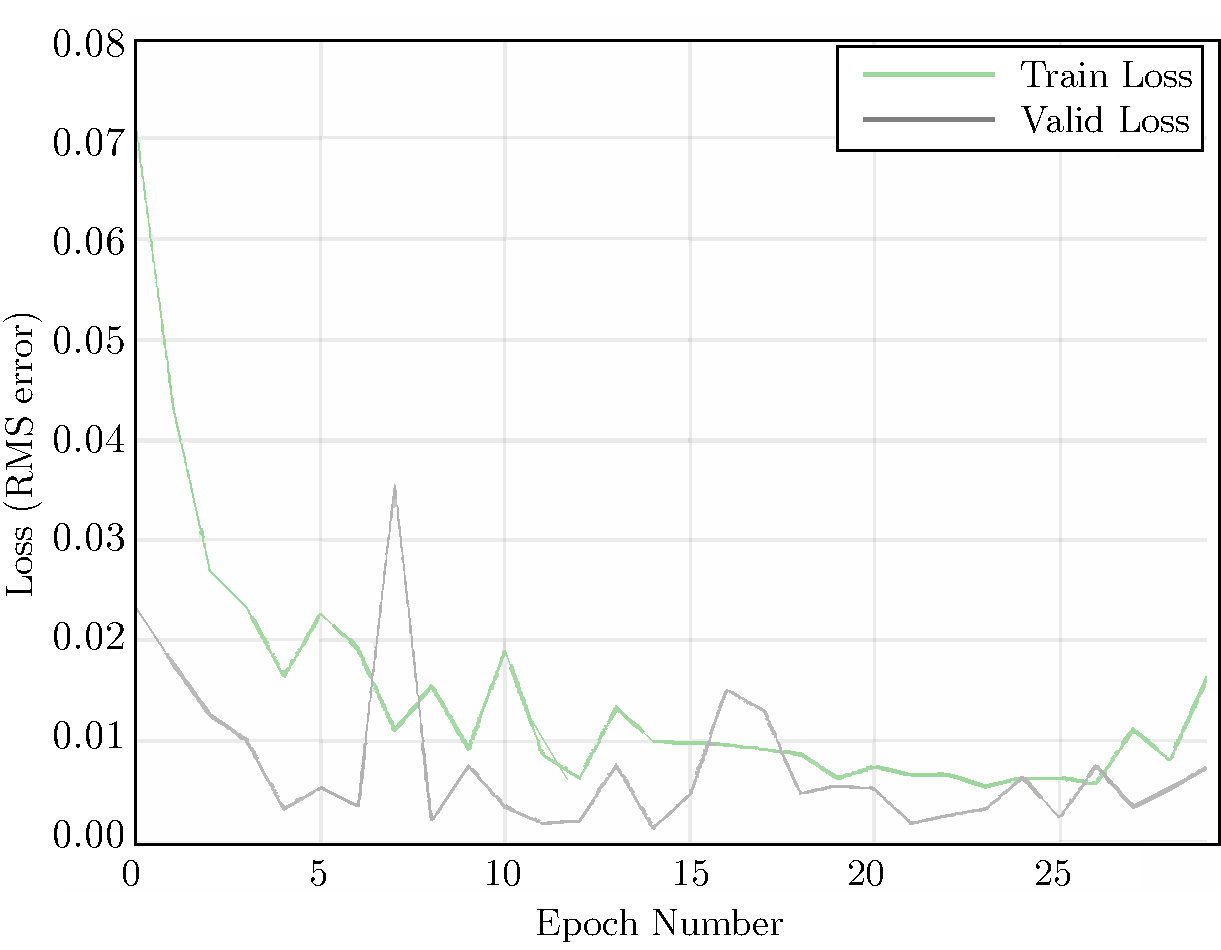
\includegraphics[width=0.6\textwidth]{trainloss.pdf}
\caption{Training and validation loss during training of the ConvNet}
\label{fig:trainloss}
\end{center}
\end{figure}

\section{Results and Discussion}

\begin{figure}[!ht]
\centering
\begin{subfigure}[b]{0.5\linewidth}
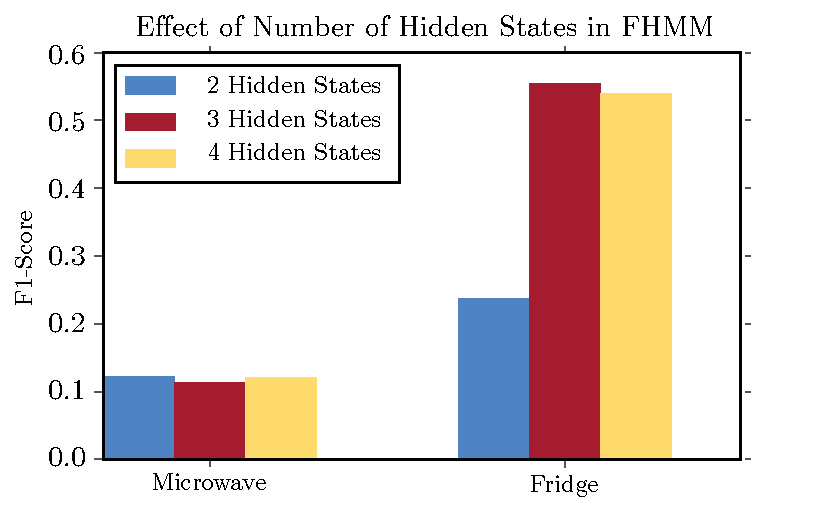
\includegraphics[width=\linewidth]{num_states.pdf}
\caption{Example of input and output of the ConvNet algorithm.}
\label{fig:FHMM_states}
\end{subfigure}%
\quad
\begin{subfigure}[b]{0.45\linewidth}
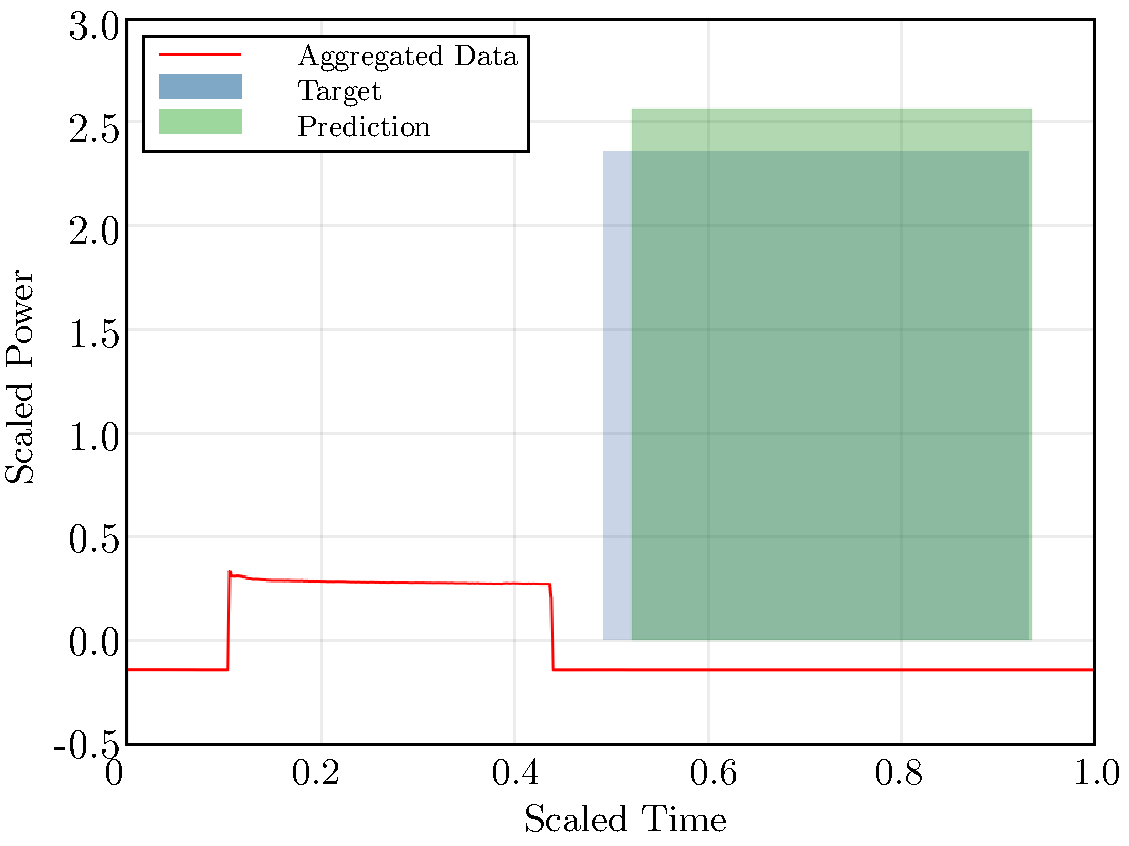
\includegraphics[width=\linewidth]{output_example.pdf}
\caption{Example of input and output of the ConvNet algorithm.}
\label{fig:convnet_result}
\end{subfigure}%
\end{figure}


The disaggregation in the case of CO is not very accurate and tracking appliances with very low energy consumption such as lights is very difficult. Appliances with relatively high and constant power consumption such as the fridge are easier to disaggregate and this explains the reason why the scores for the microwave are substantially lower in the case of CO. Disaggregation scores for Combinatorial Optimization can be improved by including more states in the training section allowing for a better modeling of each appliance but it is also accompanied by a computational cost that scales exponentially with the number of states.

We find that for the FHMM, increasing the number of hidden states from 2 to 3 improved the f1-score for fridge, but had little effect on the microwave. Further increasing the number of hidden states to 4 had only a small effect for both fridge and microwave. An FHMM with 2 hidden states will have one state representing the appliance being off and one state representing the appliance being on. The third state can represent the appliance operating at a lower power level, such as spin and fill cycles of a washing machine. In this case of the microwave, the appliance likely operates only at one power setting and increasing the number of hidden states does not improve the model.

The ConvNet outperformed the other algorithms for the fridge and the microwave in terms of the F$_1$-score, accuracy and recall. It is quite astonishing that the model can recognize from the input shown in Figure~\ref{fig:convnet_result} the activation of the fridge that starts after the bump in the aggregated data. Instead of training one algorithm per appliance we could have increased the number of output neurons to 6 and train for the start time, end time and average power of the two appliances at the same time.

\begin{figure}[!ht]
  \centering
  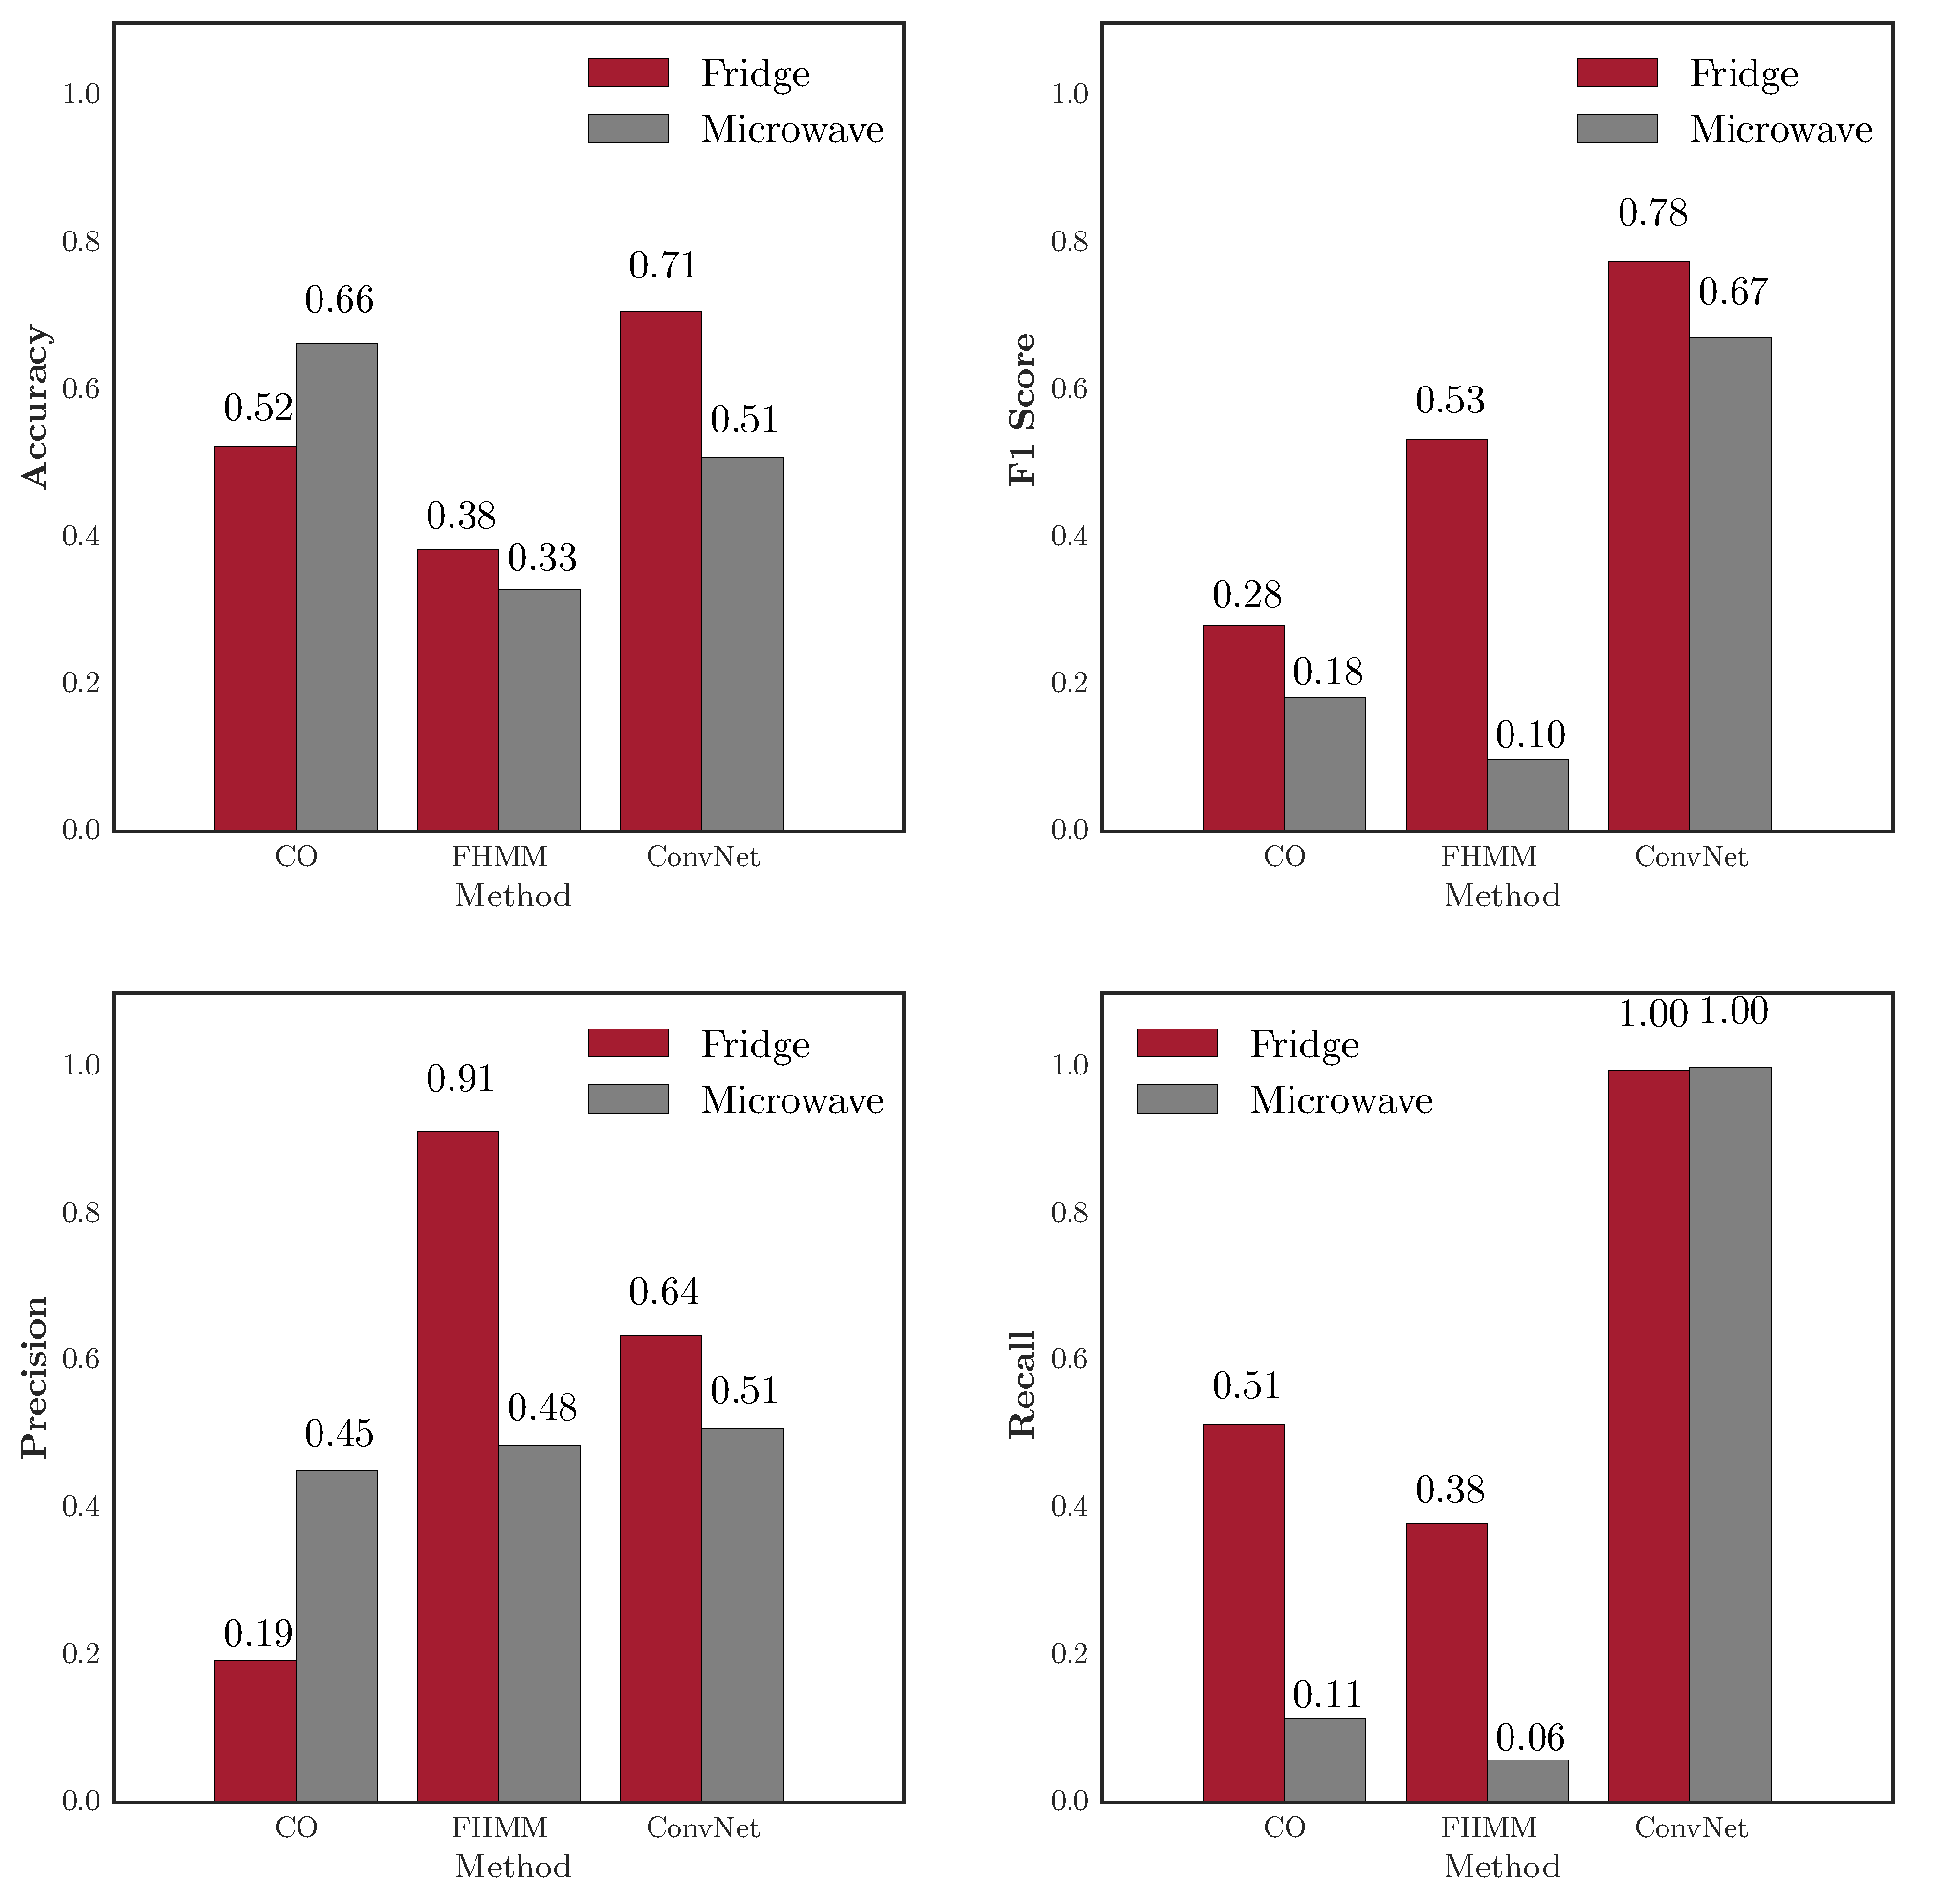
\includegraphics[width=0.8\textwidth]{Scores}
  \caption{The Accuracy, F1, Recall and Precision Scores for each method used for Disaggregation and per appliance
disaggregated}\label{fig:scores}
\end{figure}
%

\section{Conclusion}
Appliance based energy disaggregation is a complicated problem if it is to be performed on data from actual households over long periods of time and for a wide class of appliances. The disaggregation efficiency of deterministic methods commonly employed in these types of problems such as Combinatorial Optimization is extremely poor and the computational cost significant. Stochastic methods are certainly much more capable in these types of problems and the metrics corresponding to the Factorial Hidden Markov Model underline this point. The computational cost for FHMM is even more significant than that of CO which suggests that even FHMM is not suitable for disaggregation over large data sets. In contrast, the efficiency achieved by the Convolutional Neural Network outperforms all other methods in every metric and is ideal for these types of problems. Analysis performed by members of our team indicates that the neural network is capable of achieving high accuracy disaggregation even with a few layers. Training takes approximately 1 hour for Neural Nets (against 30 seconds for FHMM) but the network, once trained, is able to disaggregate fairly quickly and certainly much quicker than CO and FHMM.


\bibliographystyle{agufull08}
\begin{thebibliography}{9999}
\bibitem{NILMTK}
Batra, N. Kelly, J. Parson, O. Dutta, H. Knottenbelt, W. Rogers, A. Singh, A. Srivastava, M., (2014),NILMTK: An Open Source Toolkit for Non-intrusive Load Monitoring, \textit{Int. Conference on Future Energy Systems}, Cambridge, UK
\bibitem{Ghahraani}
Ghahramani, Z., Jordan, M.J. (1997), Factorial Hidden Markov Models, \textit{Machine Learning}, 29, 245-273.
\bibitem{Neural_Kelly}
Kelly, J. Knottenbelt, W. (2015), Neural NILM: Deep Neural Networks Applied to Energy Diseggragation,\textit{ACM BuildSys'15}, Seoul
\bibitem{Hart1985}
Hart G. W. (1985), Prototype nonintrusive appliance load monitor. Technical report, MIT Energy Laboratory and Electric Power Research Institute, Sept. 1985.
\bibitem{Hart}
Hart G. W. (1992), Nonintrusive Appliance Load Monitoring, \textit{Proceedings of the IEEE}, (80)12
\bibitem{REDD}
Kolter, J.Z. Johnson, M.J. (2011), REDD: A Public Data Set for Energy Disaggregation Research, \textit{SustKDD 2011}, San Diego, CA, USA
\bibitem{Adam}
Kingma, D.P., Ba, J.L. (2015), ADAM: A Method for Stochastic Optimization, \textit{ICLR 2015}, San Di    ego, CA, USA.
\end{thebibliography}

\end{document}
